\section{Method}
\subsection{Problem Setup}
An input sample is $(I,T)$, where $I$ is an RGB image and $T$ is a grasping
instruction.  Ground-truth rectangles are converted into dense maps
$\mathrm{pos}$, $\cos(2\theta)$, $\sin(2\theta)$, and normalized
$\mathrm{width}$; post-processing decodes the predicted dense maps into a
rectangle.

\subsection{Clean LGDM Baseline}
LGDM computes $y_{\mathrm{view}}\in\mathbb{R}^{8\times19\times19}$ with
ALBEF, but the released decoder does not use it, and the upstream training
script does not back-propagate the diffusion loss.  Our baseline keeps the
official decoder structure and optimizes
\begin{equation}
  \mathcal{L}_{\mathrm{base}} =
  \mathcal{L}_{\mathrm{diffusion}}
  + \mathcal{L}_{\cos}
  + \mathcal{L}_{\sin}
  + \mathcal{L}_{\mathrm{width}}.
  \label{eq:base}
\end{equation}
We also re-enable a raw ``plain-$y$'' injection into the GG-CNN decoder
feature $F_v$ for the language-conditioning ablation.

\subsection{LSAR}
Semantic alignment does not identify which part of a target affords a grasp.
LSAR combines the decoder feature with the language map and learns a small
residual:
\begin{align}
  Z &= \mathrm{concat}\bigl(F_v,\ y_{\mathrm{view}}\bigr), \\
  H &= \mathrm{ReLU}\bigl(\mathrm{conv}_{3\times3}(
        \mathrm{GN}(\mathrm{ReLU}(
          \mathrm{conv}_{3\times3}(Z))))\bigr), \\
  \Delta &= s\,\mathrm{conv}_{1\times1}(H), \\
  F' &= \mathrm{ReLU}\bigl(F_v+\Delta\bigr).
\end{align}
We fix $s=0.01$ to keep the residual perturbation small.  The module also
emits a $19\times19$ affordance map
$A=\mathrm{conv}_{1\times1}(H)$ for an auxiliary term studied below.

\begin{figure}[t]
\centering
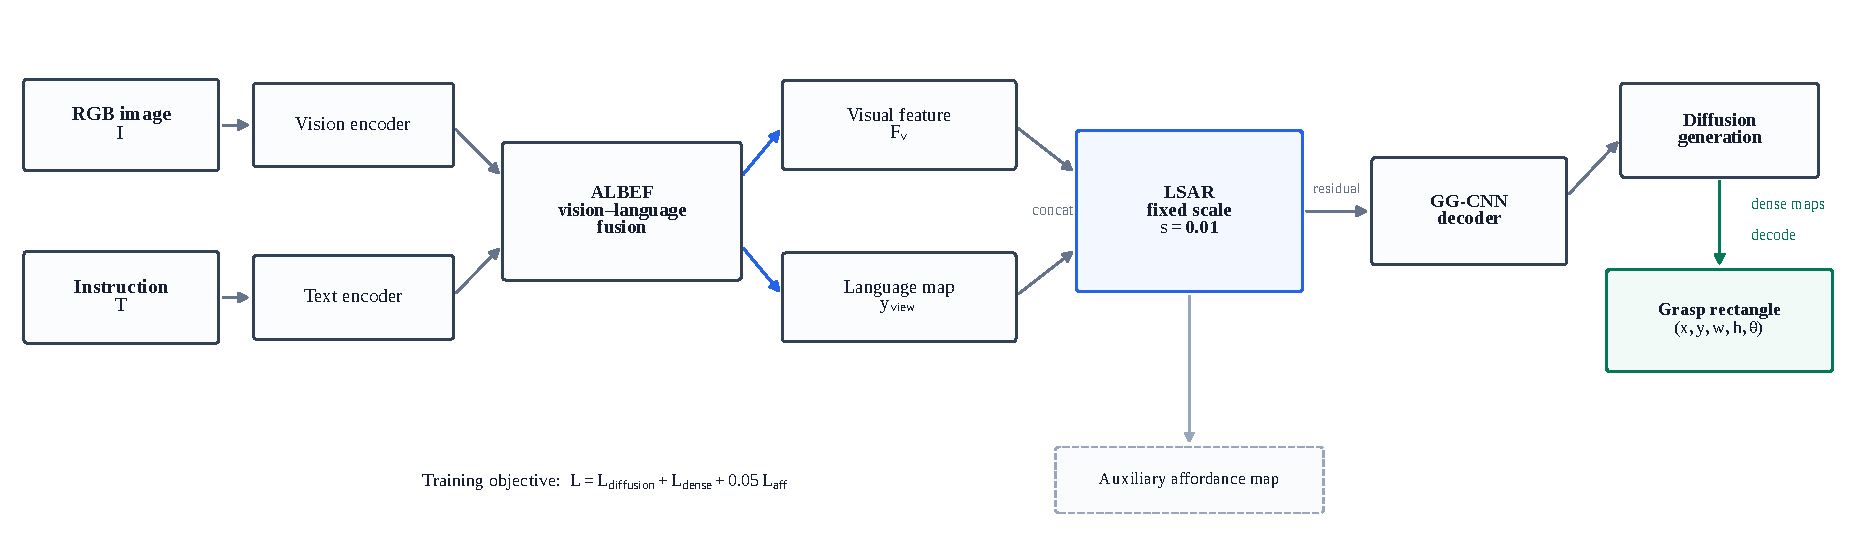
\includegraphics[width=0.98\linewidth]{figures/architecture.pdf}
\caption{Pipeline: ALBEF fusion, LSAR residual injection, GG-CNN decoding, and
diffusion grasp generation.}
\label{fig:arch}
\end{figure}

\subsection{Training Objective}
The final objective is
\begin{equation}
  \mathcal{L}=\mathcal{L}_{\mathrm{base}}
  + \lambda_{\mathrm{aff}}\,
    \mathrm{MSE}\Bigl(A,\ \mathrm{AdaptiveAvgPool}_{19}(\mathrm{pos})\Bigr),
  \label{eq:loss}
\end{equation}
with $\lambda_{\mathrm{aff}}=0.05$ in the final method.
